%%%%%%%%%%%%%%%%%%%%%%%%%%%%%%%%%%%%%%%%%%%%%%%%%%%%%%%%%%%%%%%%%%%%%%%%%%%%%%%%
%\section{Review of the LaMET Approach}\label{sec:LaMET}
%%%%%%%%%%%%%%%%%%%%%%%%%%%%%%%%%%%%%%%%%%%%%%%%%%%%%%%%%%%%%%%%%%%%%%%%%%%%%%%%

The original definition of the parton distribution function (PDF) of a
hadron with momentum $P=(P_0,0,0,P_z)$ depends on the correlator
of the quark bilinear operator defined on a lightcone:
%
\begin{equation}
h(\xi \lambda \cdot P) \equiv
  \frac{1}{2\lambda \cdot P}
  \left\langle P \left\vert
    \bar{\psi}(0) \lambda \cdot \gamma
    \Gamma \left(0,\xi \lambda \right) \psi(\xi \lambda)
  \right\vert P \right\rangle,  \label{eq:h-definition}
\end{equation}
%
where $\psi$ is the quark field operator, $\lambda=(1,0,0,-1)/\sqrt{2}$
is a lightlike vector with $\lambda^2=0$, $\gamma$ is the Dirac
matrix and the gauge link is
%
\begin{equation}
\Gamma \left( \zeta \lambda , \eta \lambda \right) \equiv
  \exp \left( ig \int_\eta^\zeta d\rho\,\lambda \cdot A(\rho \lambda) \right)
\end{equation}
%
with $g$ the strong coupling constant and $A$ the gauge field.
$h\left(0\right)$ is normalized to the total quark number of the hadron.
The physical PDF $q(x)$ of the hadron is the Fourier transform of $h$:
%
\begin{equation}
q(x,\mu) \equiv
  \int_{-\infty}^\infty \frac{d\xi \,\lambda \cdot P}{2\pi}
    e^{+ix \xi \lambda \cdot P} h(\xi \lambda \cdot P),  \label{one}
\end{equation}
%
where $\mu$ is the renormalization scale. This definition is invariant
under a boost along the $z$-direction. In particular, it is valid
in the rest frame where $P_z=0$.

Under the operator product expansion,
%
\begin{equation}
h \simeq
  \frac{1}{2\lambda \cdot P}
  \sum_{n=1}^\infty
    \frac{\left( -i\xi \right)^{n-1}}{\left( n-1 \right)!}
    \left\langle P \left\vert
    \bar{\psi}(0) \lambda \cdot \gamma \left( i\lambda \cdot D\right)^{n-1} \psi(0)
    \right\vert P\right\rangle,
\end{equation}
%
with $D$ the covariant derivative and higher-twist terms neglected.
The operator can be written as
%
\begin{eqnarray}
\bar{\psi} \lambda \cdot \gamma \left( i\lambda \cdot D\right)^{n-1} \psi &=&
  \lambda_{\mu_1} \cdots \lambda_{\mu_n} O^{\{\mu_1\cdots \mu_n\}},  \label{O1} \\
O^{\{\mu_1\cdots \mu_n\}} &=&
  \bar{\psi} \gamma^{\{\mu_1}iD^{\mu_2}\cdots iD^{\mu_n\}} \psi ,  \label{O2}
\end{eqnarray}
%
where $\{...\}$ indicates symmetrization of the enclosed indices.
The tensor $\lambda_{\mu_1}\cdots \lambda_{\mu_n}$ is symmetric and
hence only the symmetric part of $O$ will contribute to the PDF.

Furthermore, since $\lambda^2=0$, the tensor $\lambda_{\mu_1}\cdots
\lambda_{\mu_n}$ is automatically traceless. For example, for $n=2$ we can write
$\lambda_{\mu_1}\lambda_{\mu_2}=\left( \lambda_{\mu_1}\lambda_{\mu_2}-g_{\mu_1\mu_2}\lambda^2/4\right) +g_{\mu_1\mu_2}\lambda^2/4$, where the first term is symmetric and traceless while the second
term is the trace term. It is clear that the trace part vanishes when $\lambda^2=0$.
Therefore, only the symmetric and traceless part of $O^{\{\mu_1\cdots \mu_n\}}$ contributes in Eq.~\ref{O1}. This symmetric and traceless operator
is a twist-2 operator whose matrix element is related to moment of the parton
distribution $a_n = \int_{-1}^1 dx\,x^{n-1} q(x)$ and $q(-x) = -\bar{q}(x)$ with
%
\begin{equation}
\left\langle P \left\vert O^{\{\mu_1\cdots \mu_n\}}-\text{traces}%
\right\vert P\right\rangle =2a_n\left( P^{\mu_1}\cdots P^{\mu_n}-%
\text{traces}\right) .  \label{O3}
\end{equation}
%
One can check easily that with Eqs.~\ref{O1}--\ref{O3}, Eq.~\ref{one} is
indeed satisfied.

The definition in Eq.~\ref{one} cannot be used to compute the PDF in
Euclidean space. Spacetime points on a lightcone in Minkowski space
satisfy the equation $t^2-\mathbf{r}^2=0$. This equation becomes
$-t_E^2-\mathbf{r}^2=0$ in Euclidean space, which is only satisfied by
the point at the origin. Therefore, the quark bilinear operator
defined on a lightcone in Minkowski space becomes a local operator in
Euclidean space, which is not desirable; Eq.~\ref{one} yields
$q(x) \propto \delta(x)$ in this case.

In principle, one can use the twist-2 operators in Eq.~\ref{O3} to recover
the PDF, provided all the moments of the PDF can be computed. However,
in practice one can only obtain the first three moments because of the
difficulty to reliably subtract the power divergence arising from
mixing of higher moments with lower ones.

If we change $\lambda$ slightly away from the lightcone to make
it spacelike ($\lambda^2<0$) while proton is still at rest, we can boost the system such that $\lambda$ is equal-time.
In other words, the following two descriptions are
identical configurations seen in different Lorentz frames: 
%
\begin{equation}
P_z=0,\,\lambda=(\beta\gamma,0,0,-\gamma) \ \text{with}\  \beta\to 1 \quad \Leftrightarrow \quad
P_z\rightarrow \infty,\,\lambda = (0,0,0,-1)
\end{equation}
%
with $\gamma = 1/\sqrt{1-\beta^2}$.  
$P_z$ characterizes the hadronic state while $\lambda$ characterizes the quark bilinear operator.

Ref.~\cite{Ji:2013dva} exploited the above relation and proposed a method to
compute PDFs on a Euclidean lattice in the following steps (illustrated in Fig.~\ref{steps}):
%
\begin{align}
\label{eq:steps}
\hspace{2in}\text{(a)}\ P_z &=\text{finite},&   \lambda&=(0,0,0,-1)  \hspace{2in}\nonumber\\
\hspace{2in}\text{(b)}\ P_z &\rightarrow \infty,&   \lambda&=(0,0,0,-1) \hspace{2in}\nonumber\\
\hspace{2in}\text{(c)}\ P_z &=0,&   \lambda&=(\beta\gamma,0,0,-\gamma)  \ \text{with}\  \beta\to 1\nonumber\hspace{2in}\\
\hspace{2in}\text{(d)}\ P_z &=0,&  \lambda^2&=0 \hspace{2in}\nonumber\\
\hspace{2in}\mbox{ or }P_z &\rightarrow\infty,& \lambda^2&=0. \hspace{2in}
\end{align}

The first step (a) is to start from the computation of Eq.~\ref{one}
with $\lambda=(0,0,0,-1)$ and a nonzero but finite $P_z$. Note
that now the quark bilinear is equal-time, and this quantity, referred to as a
``quasi-distribution'' $\tilde{q}(x,\Lambda ,P_z)$, 
can be computed on a Euclidean lattice with an ultraviolet (UV) cutoff $\Lambda$.
With $\lambda^2 \neq 0$, $O^{\{\mu_1\cdots \mu_n\}}$ in Eq.~\ref{O1} is symmetric
but not traceless. However, its structure only differs from a twist-2 operator
by trace terms. Therefore, by Eq.~\ref{O3}, its matrix element
$\left\langle P\left\vert O^{\{\mu_1\cdots \mu_n\}}\right\vert P\right\rangle$
is still related to the moment of the PDF $a_n$ plus trace terms. As discussed in
Ref.~\cite{Ji:2013dva}, the quark-level trace contribution on the left-hand
side of Eq.~\ref{O3} is a twist-4 effect and is an
$\mathcal{O}(\Lambda_\text{QCD}^2/P_z^2)$ correction, while the trace
contribution on the right-hand side is an $\mathcal{O}(M^2/P_z^2)$ correction
with $M$ the nucleon mass. There is also an $\mathcal{O}(\alpha_s\equiv g^2/4\pi)$
quantum correction to the operator $O^{\{\mu_1\cdots \mu_n\}}$ which
could depend on $P_z$ as well. Taking into account these $P_z$-dependent
corrections, one can take $P_z\rightarrow \infty$ and go from step
(a) to step (b). From step (b) to (c), nothing needs to be done, since, as explained above, they are the same system viewed in different Lorentz frames.

Going from step (c) to step (d) is nontrivial, but one can instead go from
(b), which is identical to (c), to (d) and use the boost invariance of  $\lambda^2=0$
to bring (d) to the $P_z\rightarrow \infty$ frame. Now both (b) and (d)
have the same hadronic state with $P_z\rightarrow \infty$ but with
different quark bilinear operators: the one in (b) with $\lambda^2 < 0$
while the one in (d) with $\lambda^2=0$. From the discussion above, this
difference yields $\mathcal{O}(\Lambda_\text{QCD}^2/P_z^2)$ and
$\mathcal{O}(M^2/P_z^2)$ corrections which vanish as
$P_z\rightarrow \infty$. The remaining correction is the
$\mathcal{O}(\alpha_s)$ Wilson coefficient renormalization in the operator
product expansion of the quark bilinear. It is governed by short-distance physics
and is independent of the hadronic state. 

\begin{figure}
\begin{center}
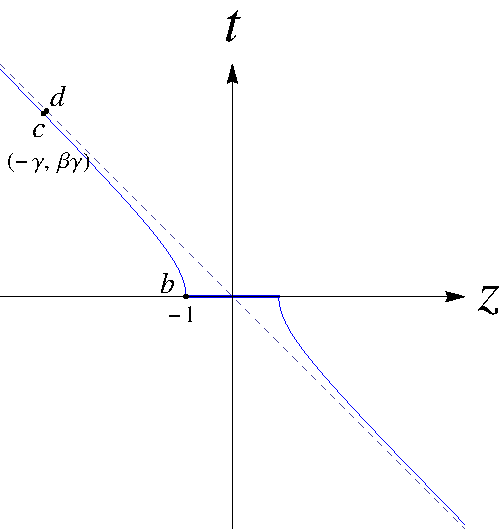
\includegraphics[width=0.24\textwidth]{images/Lorentz_boost} 
\end{center}
\caption{Illustration of the stepwise procedure in Eq.~\ref{eq:steps}.}
\label{steps}
\end{figure}


The lightlike condition $\lambda^2=0$ in (d) implies that the quark bilinear
operator is boost
invariant, and hence, the Wilson coefficient does not depend on $P_z$, but
this is not the case for (b). This is because in the former case $P_z$ is
taken above the UV cutoff and is no longer dynamical, while in the latter
case $P_z$ is below the UV cutoff and is still dynamical. The former can
be considered as an effective field theory of the latter which is analogous
to the relation between the heavy-quark effective theory (HQET) and its full
theory \cite{Ji:2014gla}. In HQET, the heavy-quark mass is taken above the
UV cutoff and is no longer a dynamical quantity while in the full theory the
heavy-quark mass is below the UV cutoff and is dynamical. The difference
between the two theories are compensated by higher-dimensional operators or
counterterms in the effective field theory which encode the short-distance
physics of the full theory that is integrated out in the effective theory.
This ``matching'' procedure can be
implemented order by order in powers of $\alpha_s$ in perturbation theory.

Summarizing the above discussion, the quasi-distribution $\tilde{q}(x,\Lambda,P_z)$,
which can be computed in Euclidean space with $\lambda=(0,0,0,-1)$
and nucleon momentum $P_z$, can be related to the $P_z$-independent
physical distribution $q(y,\mu)$ with $\lambda=(1,0,0,-1)/\sqrt{2}$ through~\cite{Ji:2013dva}
%
\begin{equation}
\tilde{q}(x,\Lambda ,P_z) = 
  \int \frac{dy}{\left\vert y\right\vert} 
    Z\left( \frac{x}{y}, \frac{\mu}{P_z}, \frac{\Lambda}{P_z}\right) q(y,\mu) +
  \mathcal{O}\left( \frac{\Lambda_\text{QCD}^2}{P_z^2},\frac{M^2}{P_z^2}\right) +\ldots .  \label{Z}
\end{equation}
%
where $\mu$ is the renormalization scale, usually in the $\overline{\text{MS}}$ scheme, $\Lambda$
will be set by the lattice spacing, and $Z$ is the kernel from the matching.
Here, we have concentrated on the flavor nonsinglet case such that the
mixing with the gluon PDF is not needed.
